\documentclass[11pt]{beamer}
\usepackage[spanish,es-tabla]{babel}
\usepackage{multirow}
\usepackage{animate}
\usepackage{media9}

\usetheme{metropolis}          
\setlength{\unitlength}{1cm}    
    \usetikzlibrary{positioning, arrows, shapes, automata}
    \tikzset{Node style/.style={thick, draw=black, circle, align=center, minimum width=70pt}}
    \tikzset{
      ->, 
      >=stealth, 
      node distance=7cm, 
    }
\setbeamerfont{section in toc}{size=\small}
\setbeamertemplate{section in toc}[sections numbered]
\setbeamerfont{subsection in toc}{size=\scriptsize}
\metroset{numbering=fraction}

%%%%%%%%%%%%%%%%%%%%%%%
\title{Segmentación de nadadores en piscinas con sistemas de captación de imágenes y vídeo}
\subtitle{Trabajo Fin de Grado}
\author[José Alberto Gómez García]{\textbf{Autor} José Alberto Gómez García
\and
     \\ \textbf{Director} Rafael Molina Soriano
\and
     \\ \textbf{Mentor} Fernando Pérez Bueno \\
     }

\date{\today}
\institute{
    Escuela Técnica Superior de Ingenierías Informática y de Telecomunicación \\
    Universidad de Granada
}
%%%%%%%%%%%%%%%%%%%%%%%


\begin{document}

    \maketitle
    
    \begin{frame}{Objetivo del trabajo}
        Propuesto por investigadores de la Facultad de Ciencias del Deporte de la UGR, el objetivo es proponer un modelo capaz de:
        \begin{enumerate}
            \item Detectar al nadador en una secuencia de vídeo.
            \item Extraer información del nadador detectado.
            \item Calcular la frecuencia media de nado en una determinada región de la piscina para cada split.
        \end{enumerate}
    \end{frame}
    
    \begin{frame}{Índice}
        \setcounter{tocdepth}{2}
        \setcounter{secnumdepth}{2}
        \tableofcontents
    \end{frame}
    
    %%%%%%%%%%%%%%%%%%%%%%%         
    \section{Estado del arte}
    \begin{frame}{Trabajos anteriores I}
        \begin{itemize}
            \item Cálculo de la frecuencia media de nado a partir de sensores adheridos al nadador.
            \item Detección de movimiento mediante algoritmos de sustracción de fondos.
            \item Detección de posiciones clave del nadador mediante redes neuronales. 
        \end{itemize}
    \end{frame}
    
    \begin{frame}{Trabajos anteriores II}
         La mayoría de trabajos que hacen uso de vídeos se centran sólo en el reconocimiento, y no en la obtención de métricas del desempeño deportivo.
    \end{frame}
    
    %%%%%%%%%%%%%%%%%%%%%%%
    \section{Sistema de captación de vídeo}
    \begin{frame}{Descripción del sistema}
        \begin{itemize}
            \item Sistema de 8 cámaras IP sobre la piscina de la Facultad de Ciencias del Deporte de la UGR.
            \item Se dispone de un plano cenital de la piscina mediante video stitching.
            \item Se genera un vídeo con resolución habitual de 1292x816 píxeles y una tasa de 41.66 FPS.
        \end{itemize}
    \end{frame}

    \begin{frame}{Fotograma generado}
        \begin{figure}
            \centering
            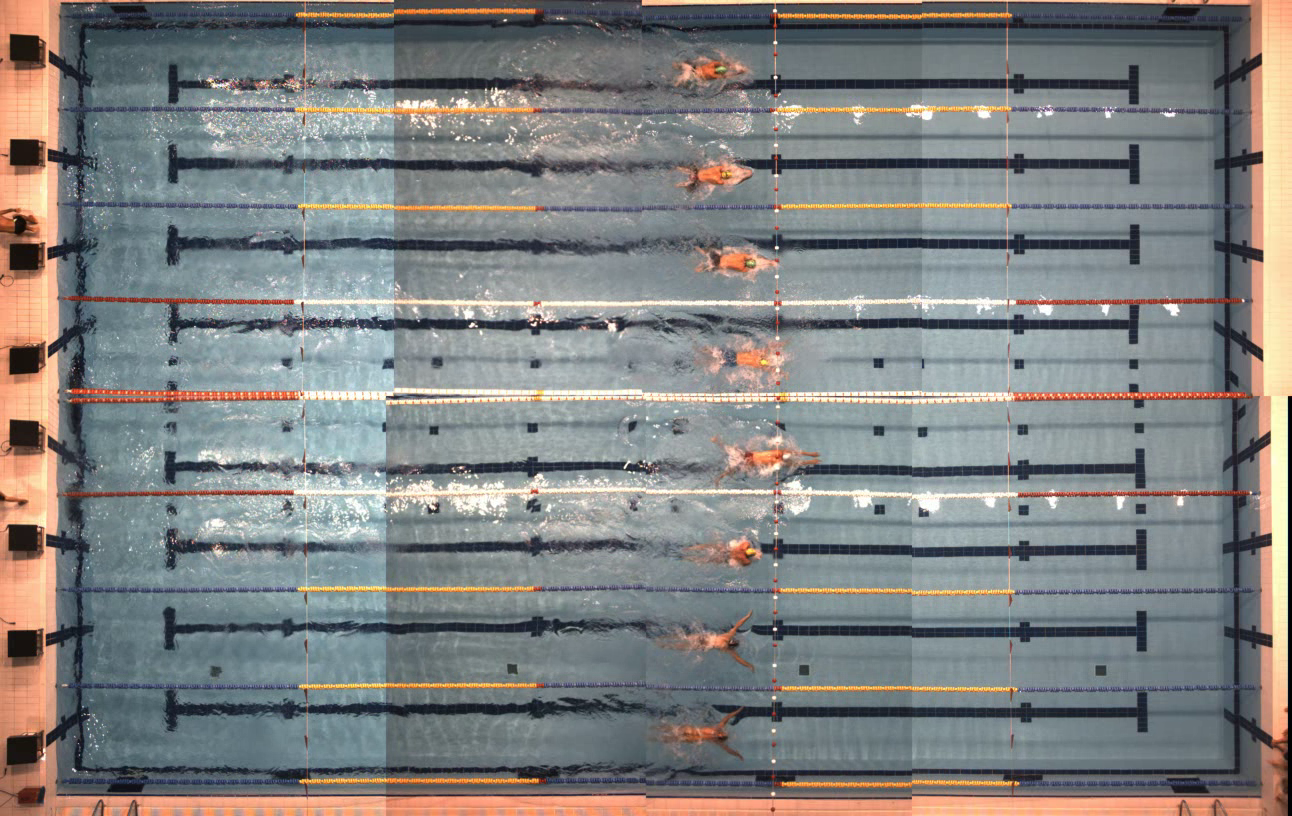
\includegraphics[scale=0.2]{imagenes/piscina_completa.png}
            \caption{Fotograma generado por el sistema de cámaras.}
            \label{fig:piscinacompleta}
        \end{figure}
    \end{frame}
    
    %%%%%%%%%%%%%%%%%%%%%%%
    \section{¿Cómo detectar al nadador?}
        \begin{frame}{Enfoques seguidos}
            Para llevar a cabo esta tarea se han seguido dos enfoques:
            \begin{itemize}
                \item Técnicas clásicas del procesamiento de imágenes.
                \item Técnicas basadas en aprendizaje profundo.
            \end{itemize}
        \end{frame}
    
        %%%%%%%%%%%%%%%%%%%%%%%
        \subsection{Técnicas clásicas del procesamiento de imágenes}
        \section*{Técnicas clásicas del procesamiento de imágenes}

        \subsubsection{Espacios de color I}
        \begin{frame}{Espacios de color}
            Una correcta elección del espacio de color puede facilitar el procesamiento.

            Se han considerado tres espacios de color:
            \begin{itemize}
                \item RGB
                \item HSV
                \item YCbCr
            \end{itemize}
        \end{frame}
        
        \begin{frame}{Espacios de color II}
        
            \begin{figure}[h!]
                \centering
                \footnotesize
                \begin{tabular}{cc}
                    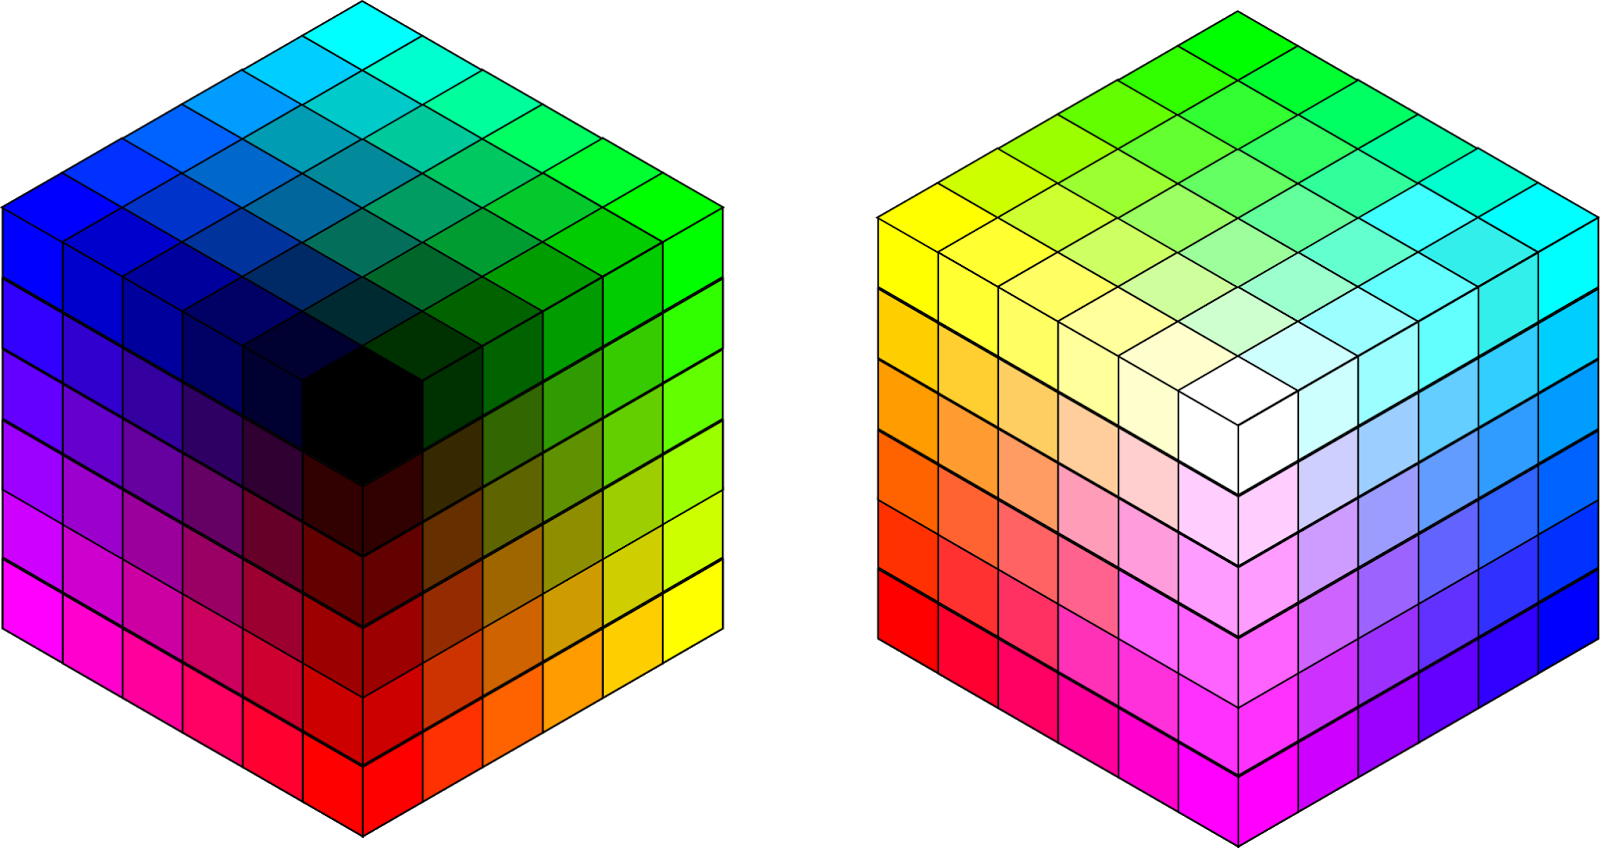
\includegraphics[height=0.27\textwidth,keepaspectratio]{imagenes/cubos_rgb.png} &
                    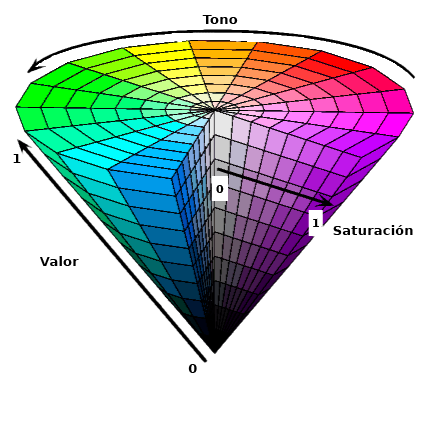
\includegraphics[height=0.27\textwidth,keepaspectratio]{imagenes/cono_hsv.png} \\
                    
                    a) Representación del espacio RGB & b) Representación del espacio HSV
                \end{tabular}
            \end{figure}
        
            \begin{figure}[h!]
                \centering
                \footnotesize
                \begin{tabular}{ccc}
                    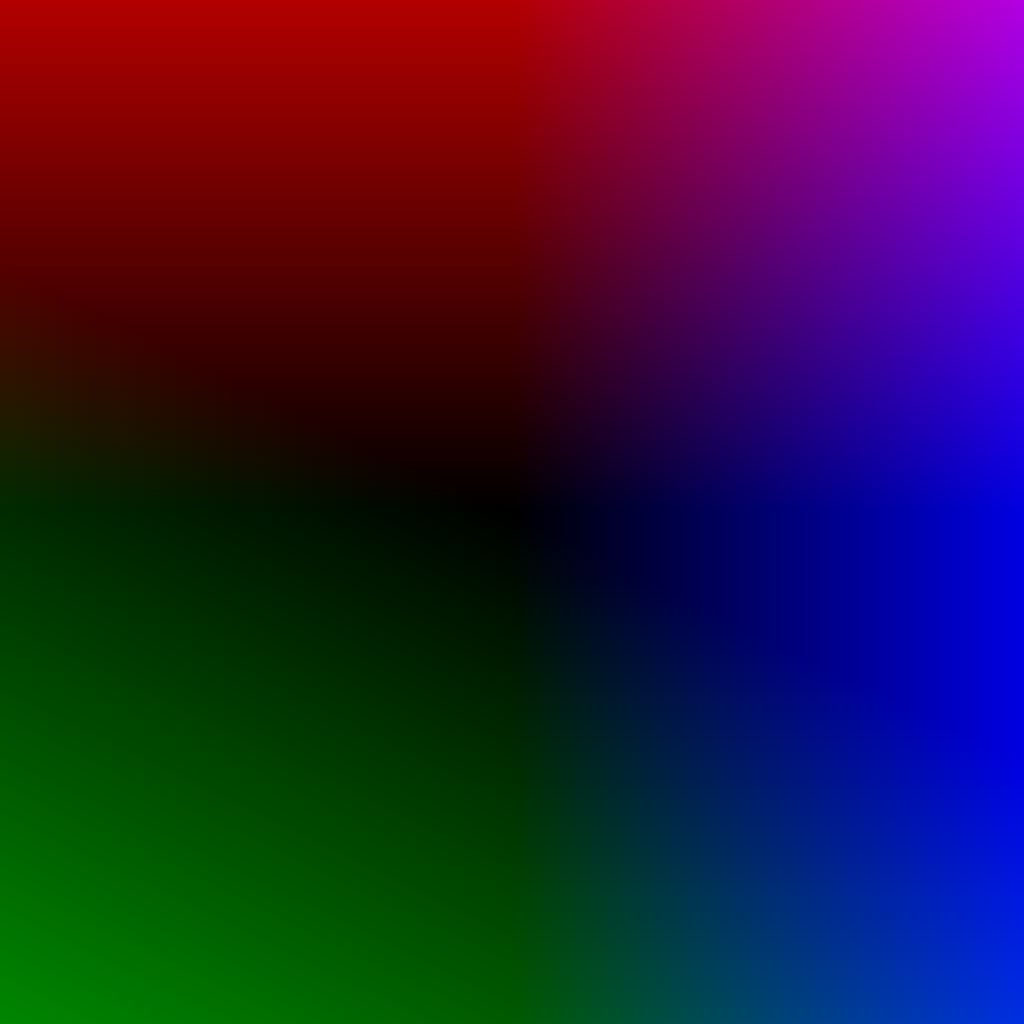
\includegraphics[height=0.25\textheight,keepaspectratio]{imagenes/YCbCr_Y0.png} & 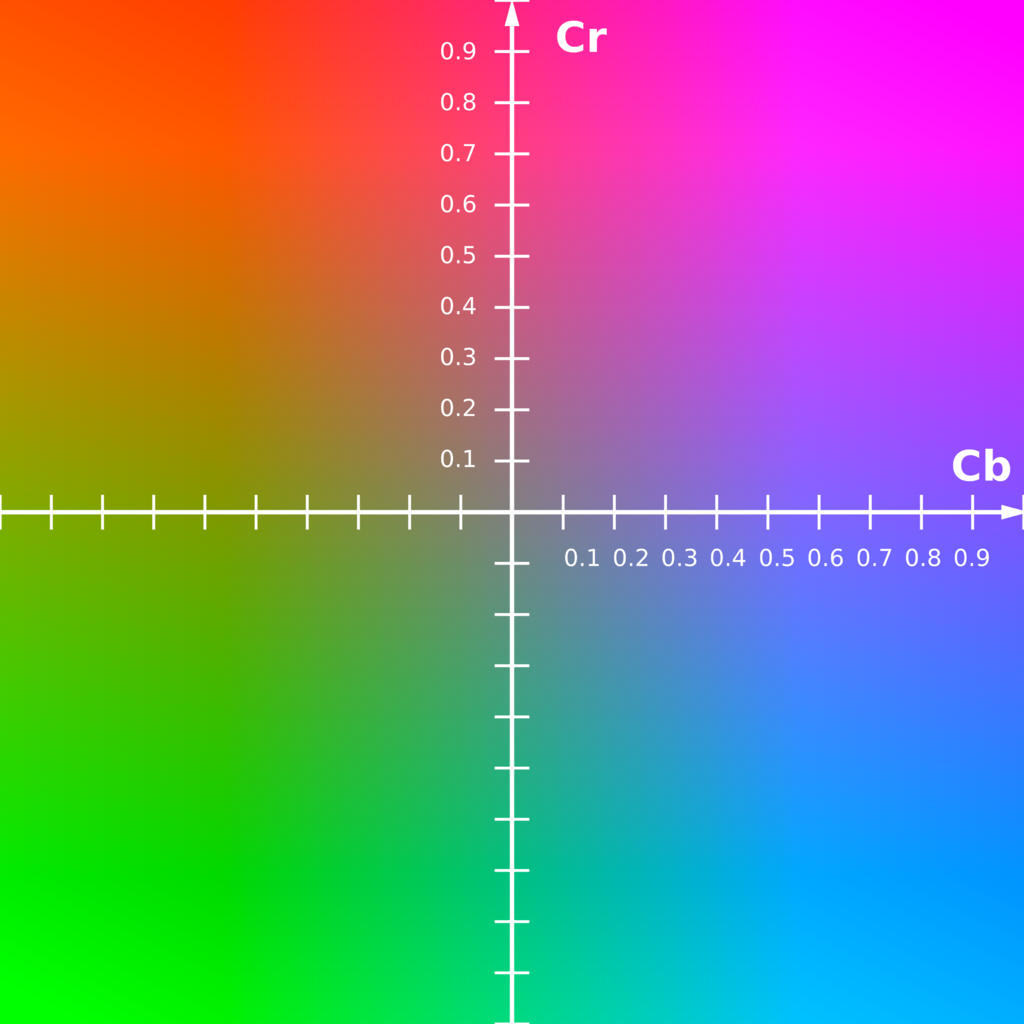
\includegraphics[height=0.25\textheight,keepaspectratio]{imagenes/YCbCr_Y50.png} &
                    
\includegraphics[height=0.25\textheight,keepaspectratio]{imagenes/YCbCr_Y100.png} \\
                \end{tabular}
                \begin{tabular}{c}
                     c) Planos Cb/Cr para diferentes luminancias (YCbCr).
                \end{tabular}
            \end{figure}
        \end{frame}
        
        \subsubsection{Ejemplos para diferentes espacios de color}
        
         \begin{frame}{Fotograma en RGB}
            \begin{figure}
                \centering
                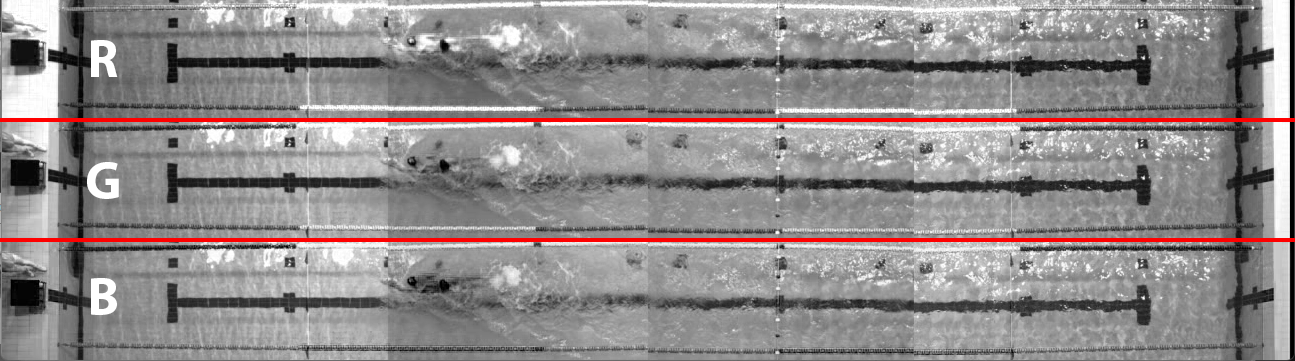
\includegraphics[scale=0.22]{imagenes/RGB_LANE.png}  
                \caption{Canales RGB por separado de una única calle de la piscina.}
                \label{fig:callergb}
            \end{figure}
             No existe una gran diferencia entre los distintos canales.
         \end{frame}
         
        \begin{frame}{Fotograma en HSV}
            \begin{figure}
                \centering
                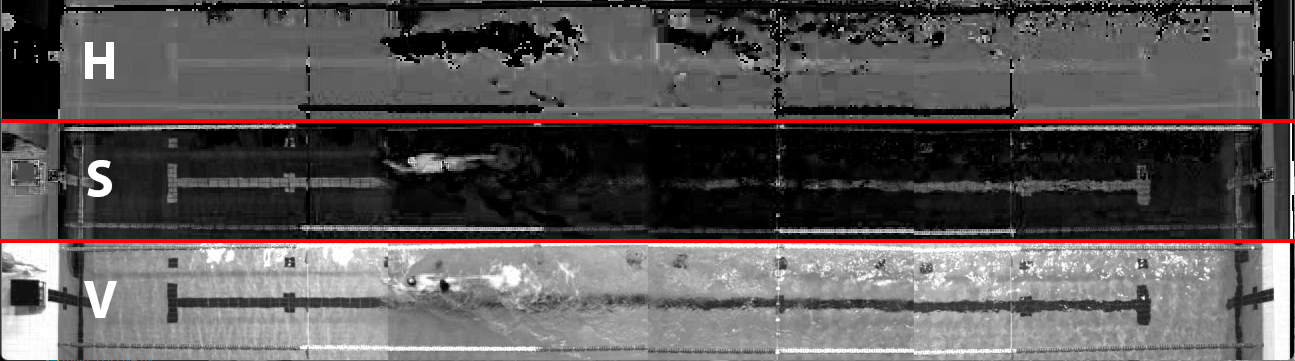
\includegraphics[scale=0.22]{imagenes/HSV_LANE.png}  
                \caption{Canales HSV por separado de una única calle de la piscina.}
                \label{fig:callehsv}
            \end{figure}
            \begin{itemize}
                \item El canal de valor es similar a los canales RGB.
                \item Con el canal de saturación el nadador se puede distinguir fácilmente.
            \end{itemize}
             
         \end{frame}
         
        \begin{frame}{Fotograma en YCbCr}
            \begin{figure}
                \centering
                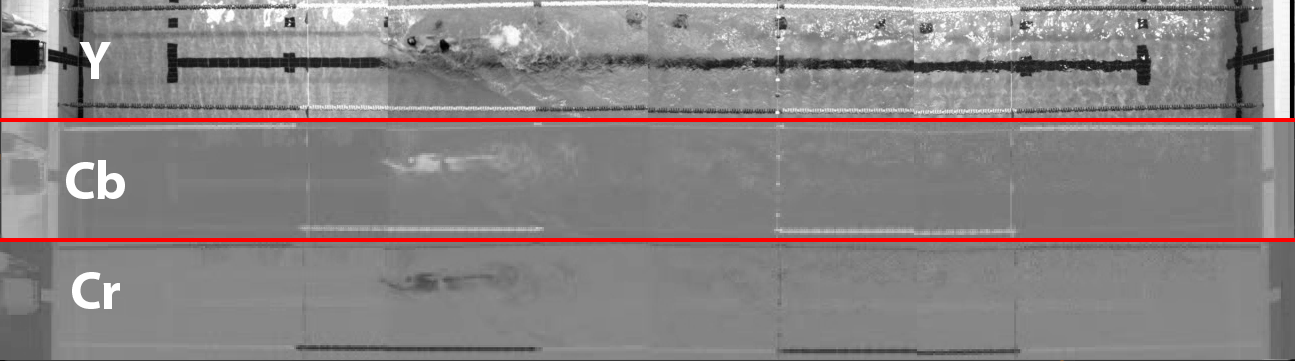
\includegraphics[scale=0.22]{imagenes/YCBCR_LANE.png}  
                \caption{Canales YCbCr por separado de una única calle de la piscina.}
                \label{fig:calleycbcr}
            \end{figure}
            \begin{itemize}
                \item El canal de luminancia es similar al canal valor de HSV y a los canales de RGB.
                \item El nadador puede reconocerse en los canales de crominancia (Cb y Cr).
            \end{itemize}
         \end{frame}
         
        \subsubsection{Algoritmos de sustracción de fondos} 
        \begin{frame}{Algoritmos de sustracción de fondos}  
            Se ha considerado el uso de tres algoritmos:
            \begin{itemize}
                \item Mezcla de gaussianas (MoG)
                \item K vecinos más cercanos (K-NN)
                \item Google Summer of Code (GSoC)
            \end{itemize}
        \end{frame}
        
        \begin{frame}{Resultado de eliminar fondo}
            El uso de los algoritmos de sustracción de fondos nos devuelven imágenes similares a:
            \begin{figure}
                \centering
                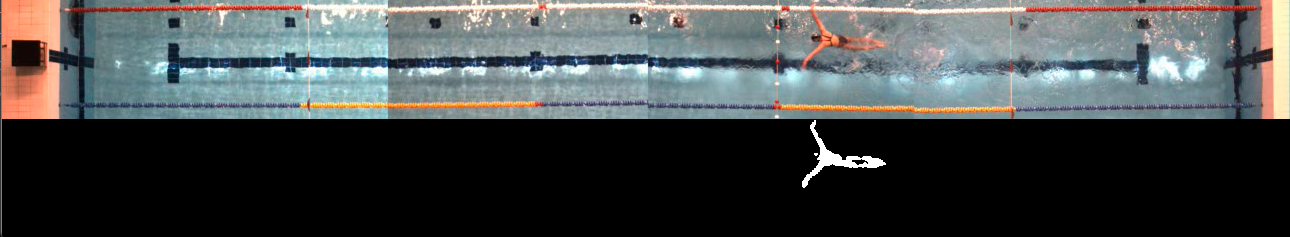
\includegraphics[scale=0.22]{imagenes/ejemplo_eliminar_fondo.png}  
                \caption{Resultado de eliminar el fondo de la imagen utilizando GSoC sobre la banda de crominancia roja de YCbCr.}
                \label{fig:ejemplosustracción}
            \end{figure}
        \end{frame}
        
        \subsubsection{Extracción y filtrado de contornos.}
        \begin{frame}{Extracción de bounding boxes}
            \begin{figure}[h!]
                \centering
                    \begin{tabular}{c}
                        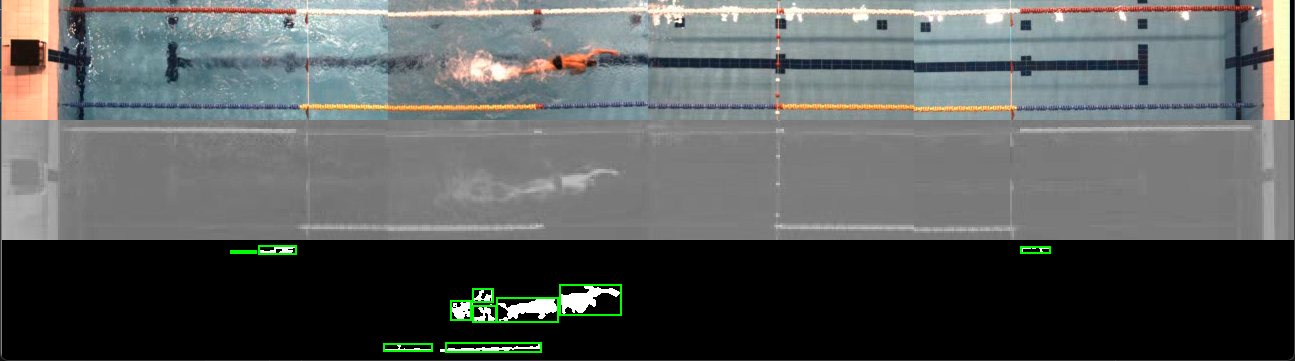
\includegraphics[scale=0.17]{imagenes/MUCHOS_CONTORNOS_I.png} \\
                        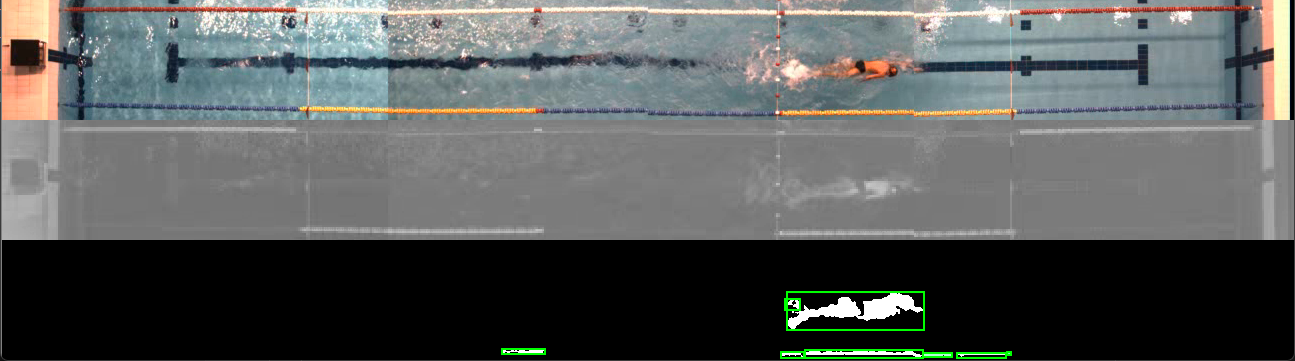
\includegraphics[scale=0.17]{imagenes/MUCHOS_CONTORNOS_III.png} 
                    \end{tabular}
                \caption{Bounding boxes detectadas sin proceso de filtrado.}
                \label{fig:muchoscontornos}
            \end{figure}
            Hay muchas cajas que no corresponden al nadador, por lo que debemos realizar un proceso de filtrado.
        \end{frame}
        
        \begin{frame}{Filtrado de bounding boxes}
        Los pasos del proceso de filtrado son siguiente:
            \begin{enumerate}
                \item Eliminar aquellas cajas que estén fuera de la piscina.
                \item Eliminar cajas en función de la altura y posición en el eje Y, para obviar las corcheras.
                \item Ordenar en función del área de manera descendente.
                \item Comprobar si las cajas de mayor área son tronco y piernas. Si lo son, unir. Si no, usar la de mayor área.
            \end{enumerate}
        Así, mantendremos la caja de mayor área, que debe corresponder al nadador.
        \end{frame}
        
        \subsubsection{Resultados experimentales}
        \begin{frame}{Métricas de segmentación}
            Necesitamos métricas para comparar cómo de buena es la detección realizada. Para ello, usaremos:
            \begin{itemize}
                \item Índice de Jaccard, o ``intersección sobre la unión''.
                     \begin{equation}
                        IoU= \frac{Area\ de\ interseccion}{Area\ de\ union} = \frac{A \cap B}{A \cup B}=\frac{A\cap B}{|A|+|B|-(A \cap B)}
                    \end{equation}
                \item Coeficiente de Sorensen-Dice, o F1-Score.
                    \begin{equation}
                        Dice = \frac{2 \times Area\ de\ interseccion}{Suma\ de\ cardinalidades} = \frac{2 \times (A \cap B)}{|A| + |B|}
                    \end{equation}
            \end{itemize}
        \end{frame}
         
        \begin{frame}{Resultados visuales}
            \begin{figure}[h!]
                \centering
                \begin{tabular}{cc}
                    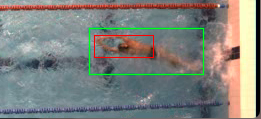
\includegraphics[width=0.43\textwidth,height=0.43\textheight,keepaspectratio]{imagenes/mala_1099.png} &
                    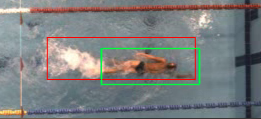
\includegraphics[width=0.43\textwidth,height=0.43\textheight,keepaspectratio]{imagenes/muchisima_agua_1014.png}
                    \\ a) IoU = 0.24; F1 = 0.38 & b) IoU = 0.40; F1 = 0.52  \\
                    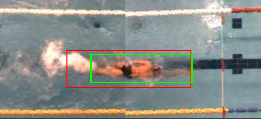
\includegraphics[width=0.43\textwidth,height=0.43\textheight,keepaspectratio]{imagenes/mucha_agua_897.png} &
                    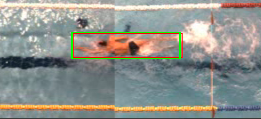
\includegraphics[width=0.43\textwidth,height=0.43\textheight,keepaspectratio]{imagenes/excelentisimo_1241.png}
                    \\ c) IoU = 0.60; F1 = 0.75  & d) IoU = 0.87; F1 = 0.93
                 \end{tabular}
                 \caption{Predicción automática (en rojo) frente a segmentación manual (en verde) para diferentes fotogramas.}
                 \label{fig:iouvisualimgs}
            \end{figure}
        \end{frame}
        
        \begin{frame}{Resultados experimentales}
            \begin{table}
                \centering
                \small
                \begin{tabular}{| c | c | c | c | c|}\hline
                    Banda & Algoritmo & IoU & Dice & T.ejecución (ms) \\ \hline
                    \multirow{3}{*}{S de HSV} & KNN  & 0.47256 & 0.56733 & 5.530 \\
                    &MOG2 & 0.49366 & 0.59887 & 5.457 \\
                    &GSoC & 0.48128 & 0.57142 & 11.778 \\ \hline
                    \multirow{3}{*}{Cb de YCbCr} & KNN  & 0.14175 & 0.22651 & \textbf{3.918} \\
                    &MOG2 & 0.39959 & 0.53033 & 4.099 \\
                    &GSoC & 0.47209 & 0.61864 & 10.939 \\ \hline
                    \multirow{3}{*}{Cr de YCbCr} & KNN  & 0.39881 & 0.55140 & 4.423 \\
                    &MOG2 & 0.56134 & 0.68497 & 4.413 \\
                    &GSoC & \textbf{0.64126} & \textbf{0.76864} & 11.051 \\ \hline
                \end{tabular}
                \caption{Comparativa de rendimiento.}
                \label{tab:rendimientofondoscap3}
            \end{table}
        \end{frame}
         
        \begin{frame}{Conclusiones}
        Extraemos las siguientes conclusiones:
            \begin{itemize}
                \item El uso de la banda de saturación de HSV permite una detección adecuada del nadador.
                \item El algoritmo GSoC suele ser el que mejores resultados proporciona, a costa de un tiempo de ejecución mayor.
                \item Los mejores resultados se consiguen haciendo uso de la banda crominancia roja de YCbCr y el algoritmo GSoC.
                \item Se satisfacen requisitos de tiempo real.
            \end{itemize}
        \end{frame}
        
        %%%%%%%%%%%%%%%%%%%%%%%
        \subsection{Técnicas basadas en aprendizaje automático}
        \section*{Técnicas basadas en aprendizaje automático}
        
        \subsubsection{Arquitecturas para la detección de objetos}
        \begin{frame}{Arquitecturas para la detección de objetos}
            Actualmente, existen varias arquitecturas para la detección de objetos:
            \begin{itemize}
                \item Region-based Convolutional Neuronal Network (R-CNN).
                \item You Only Look Once (YOLO).
                \item Single Shot Detector (SSD).
            \end{itemize}
            Se decide utilizar YOLOv4 debido a un mayor rendimiento y menor tiempo de ejecución que el resto de competidores.
        \end{frame}
        
        \subsubsection{YOLO}
        \begin{frame}{YOLO}
            \begin{itemize}
                \item Creado por Joseph Redmond en 2016, está escrito en C y CUDA. Este autor desarrolla las tres primeras versiones de la arquitectura.
                \item Es un detector de objetos de una única fase. Solo se requiere de una propagación de la imagen por la red neuronal para detectar múltiples objetos.
            \end{itemize}
        \end{frame}

        
        \subsubsection{Entrenamiento del modelo YOLOv4}
        \begin{frame}{Entrenamiento del modelo YOLOv4}
            \begin{itemize}
                \item Decidimos partir de un entrenamiento sobre el dataset MS COCO.
                \item Así, se es capaz de reconocer personas de forma general, pero no nadadores.
                \item Aplicamos ``fine tuning'' para especializar al modelo en la detección de nadadores.
            \end{itemize}
        \end{frame}
        
        \begin{frame}{Proceso de ``fine tuning'' I }
            \begin{itemize}
                \item Disponemos de un conjunto de 1970 imágenes etiquetas de nadadores.
                \item Hacemos uso del repositorio \textit{Darknet} para realizar el segundo entrenamiento. Ajustamos configuración, ejecutamos y esperamos resultados.
            \end{itemize}
            \begin{figure}[h!]
                \centering
                    \begin{tabular}{cc}
                        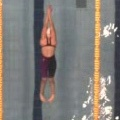
\includegraphics[scale=0.6]{imagenes/aspa_0179.jpg} &
                        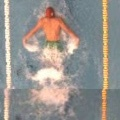
\includegraphics[scale=0.6]{imagenes/cm_428.jpg} 
                    \end{tabular}
                \caption{Ejemplo de imágenes de entrenamiento.}
                \label{fig:imagenesentrenamiento}
            \end{figure}
        \end{frame}
        
        \begin{frame}{Proceso de ``fine tuning'' II}
        Durante el entrenamiento, hubo varios problemas que resolver:
        \begin{itemize}
            \item Orientación del vídeo.
            \item No detección sobre vídeos a pesar de buenos resultados de entrenamiento.
            \item Detección sólo en una parte del vídeo.
        \end{itemize}
            
        \end{frame}
        
        \begin{frame}{Proceso de ``fine tuning'' III}
            La diferencia de dimensiones entre las imágenes de entrenamiento y el vídeo hace que no se detecte nada en los vídeos. Hay que cambiar la resolución de la red neuronal. 
            
            \begin{figure}[h!]
                \centering
                    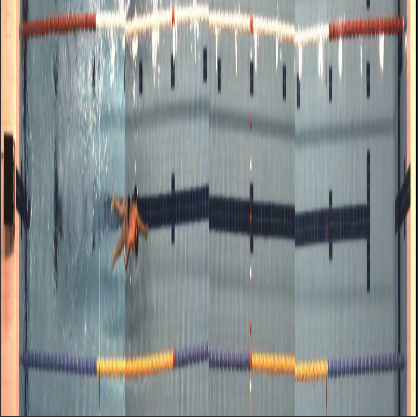
\includegraphics[width=0.43\textwidth,height=0.43\textheight,keepaspectratio]{imagenes/416x416_YOLO_resize.png}
                 \caption{Fotograma redimensionado a tamaño cuadrado.}
                 \label{fig:yolosizeexample}
            \end{figure}
            
        \end{frame}
        
        \begin{frame}{Ajuste de la resolución}
            \begin{table}
                \centering
                \scriptsize
                \begin{tabular}{| c | c | c | c | c | c | c| } \hline
                    Ancho & Alto & IoU & F1-Score & Confianza & T.ejec (ms) & R.Aspecto \\ \hline
                    416 & 416 & 0.00000 & 0.00000 & 0.000 & 19.141 & 1:1 \\
                    416 & 4480 & 0.67197 & 0.80132 & \textbf{0.968} & 140.805 & 10.77:1* \\ 
                    256 & 2688 & 0.72532 & 0.82767 & 0.818 & \textbf{54.571} & 10.5:1 \\ 
                    416 & 2112 & \textbf{0.73378} & \textbf{0.84287} & 0.907 & 67.488 & 5.077:1  \\
                    416 & 2528 & 0.71667 & 0.83191 & 0.945 & 78.505 & 6.077:1 \\ 
                    416 & 3232 & 0.70861 & 0.82610 &  0.963 & 103.808 & 7.77:1 \\ \hline
                \end{tabular}
                \caption{Métricas en función de la redimensión realizada por la red. La relación de aspecto original aparece marcada con *.}
                \label{tab:yolosizematters}
            \end{table}
            Elegimos resolución 256 x 2688.
        \end{frame}
        
        \begin{frame}{Resultados experimentales}
            \begin{table}
                \centering
                \begin{tabular}{| c | c | c | c | } \hline
                    Enfoque & IoU & F1Score  & T.ejecución (ms)  \\ \hline
                    GSoC sobre Cr & 0.64126 & 0.76864 & \textbf{11.051} \\
                    YOLOv4 & \textbf{0.72532} & \textbf{0.82767} & 54.571  \\ \hline
                \end{tabular}
                \caption{Métricas para cada aproximación.}
                \label{tab:metricasaproximaciones}
            \end{table}
        \end{frame}
        
        \begin{frame}{Conclusiones}
            \begin{itemize}
                \item El uso de YOLOv4 ofrece mejores resultados que la aproximación basada en técnicas clásicas del procesamiento de imágenes.
                \item YOLOv4 requiere un tiempo de ejecución considerablemente mayor, que no satisface requisitos de tiempo real.
            \end{itemize}
        \end{frame}
        
        \begin{frame}{Vídeo de ejemplo}
            Veamos un vídeo de ejemplo con el resultado final.
            %\begin{center}
            %    \animategraphics[controls,width=\linewidth]{20}{frames_video/frame}{0}{573}
            %\end{center}
    
        \end{frame}

    
    %%%%%%%%%%%%%%%%%%%%%%%
    \section{¿Cómo calcular la frecuencia media de nado?}  
    
        \begin{frame}{¿Qué necesitamos?}
            Necesitaremos hallar dos valores:
            \begin{itemize}
                \item Cuanto tiempo se tarda en recorrer cada split \\ -> Usaremos la coordenada X y número de fotograma.
                \item Cuantas brazadas se realizan en cada tramo \\ -> Usaremos la anchura del nadador.
            \end{itemize}
            Conocidos estos valores, se puede calcular la frecuencia media de nado para cada split.
        \end{frame}
        
        \begin{frame}{Preprocesado}
            Antes de comenzar, necesitamos preprocesar las coordenadas y anchuras que usaremos.
            \begin{itemize}
                \item Debemos tratar posibles valores nulos.
                \item Intentaremos reducir el posible ruido existente entre los valores.
            \end{itemize}
        \end{frame}
        
        %%%%%%%%%%%%%%%%%%%%%%%
        \subsection{Tiempo empleado por split}
        \begin{frame}{¿Cómo delimitar cada tramo?}
            \begin{itemize}
                \item Calcular extremos relativos. Esto permite dividir el vídeo en función del sentido del nado.
                \item Delimitar la región de interés (ROI) para cada split. 
                \item Hallar tiempo empleado en cada ROI.
            \end{itemize}
        \end{frame}
        
        \begin{frame}{Puntos de interés}
        \begin{figure}
            \centering
            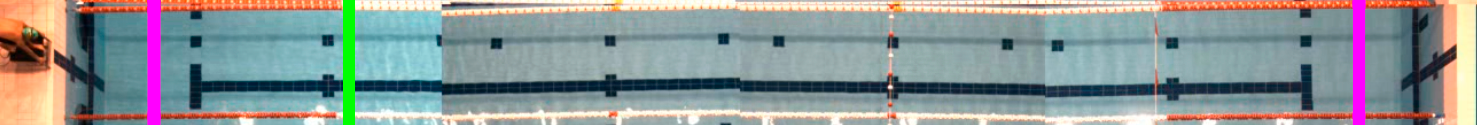
\includegraphics[scale=0.2]{imagenes/limites_ROI.png}
            \caption{Límites de la región de interés. En verde se marca el inicio de la primera ROI, en morado se marcan los extremos habituales de las ROI.}
            \label{fig:my_label}
        \end{figure}
            \begin{figure}
                \centering
                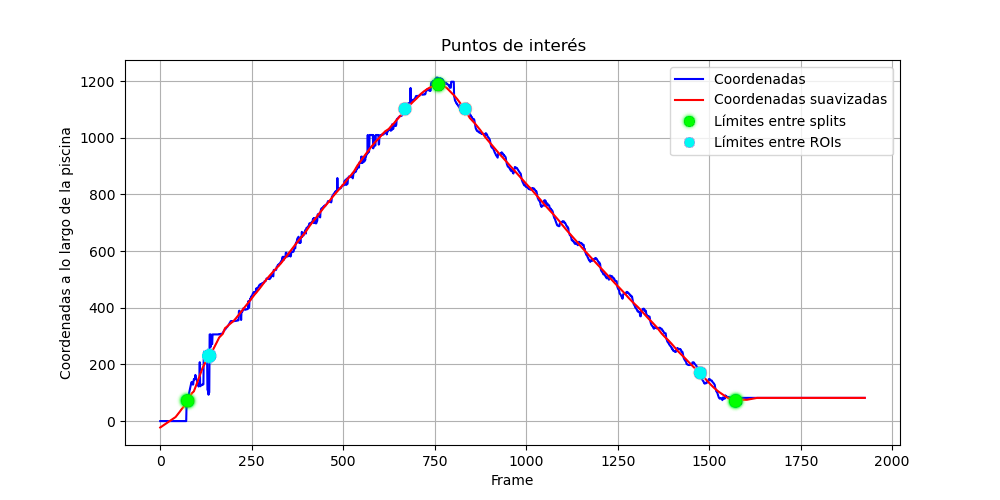
\includegraphics[scale=0.21]{imagenes/SENTID.png}
                \caption{Puntos de interés en el eje X.}
                \label{fig:puntosinteresx}
            \end{figure}
        \end{frame}
        
        \begin{frame}{Tiempo empleado por split}
            Conocidos los fotogramas en los que el nadador pasa por los extremos de la ROI, podemos calcular el tiempo empleado haciendo uso de: \\
            \begin{equation}
                    T (s) = \frac{\text{nº fotograma final ROI} - \text{nº fotograma inicial ROI}}{ \text{tasa de fotogramas por segundo}}
            \end{equation}
        \end{frame}
        
        %%%%%%%%%%%%%%%%%%%%%%%
        \subsection{Número de brazadas por split}
        
        \begin{frame}{¿Cómo detectar brazadas?}
            Para identificar los momentos en que se realiza una brazada haremos uso de la variación de anchura del nadador.
            \begin{figure}
                \centering
                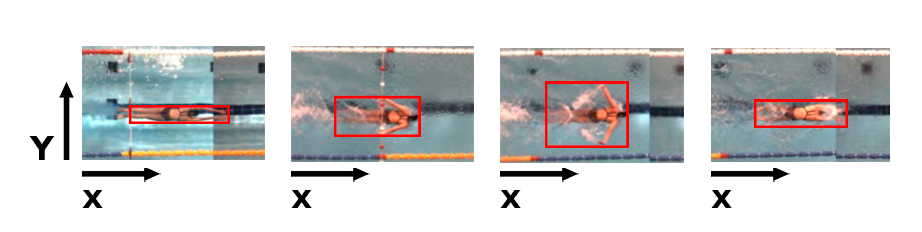
\includegraphics[scale=0.3]{imagenes/variacion_anchura_nadador.png}
                \caption{Variación de la anchura del nadador conforme nada.}
                \label{fig:variacionanchura}
            \end{figure}
        \end{frame}
        
        \begin{frame}{Detección de brazadas}
            \begin{itemize}
                \item Buscaremos máximos relativos mayores a la media.
                \item Debe existir una separación mínima entre máximos relativos.
            \end{itemize}
            \begin{figure}[h!]
                \centering
                    \begin{tabular}{cc}
                        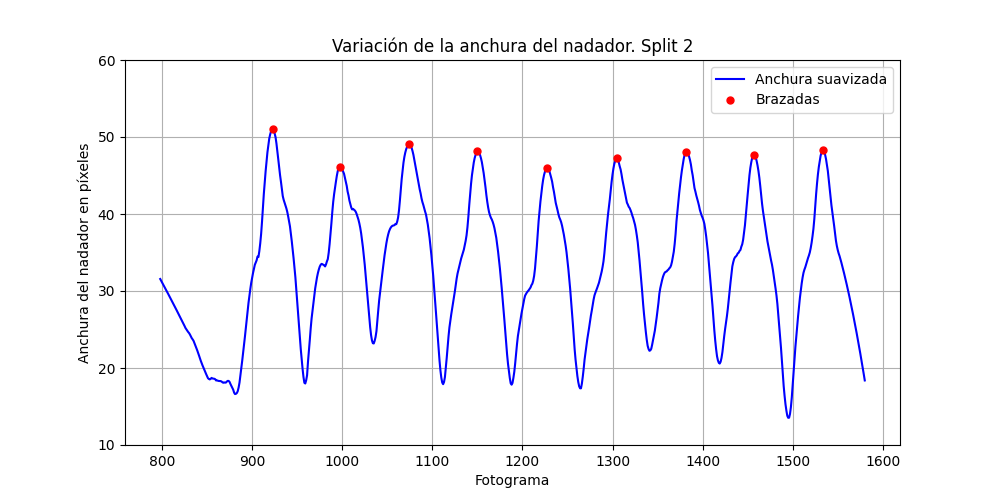
\includegraphics[scale=0.2]{imagenes/anchuras_calle_3_mariposa_YOLO.png} &
                        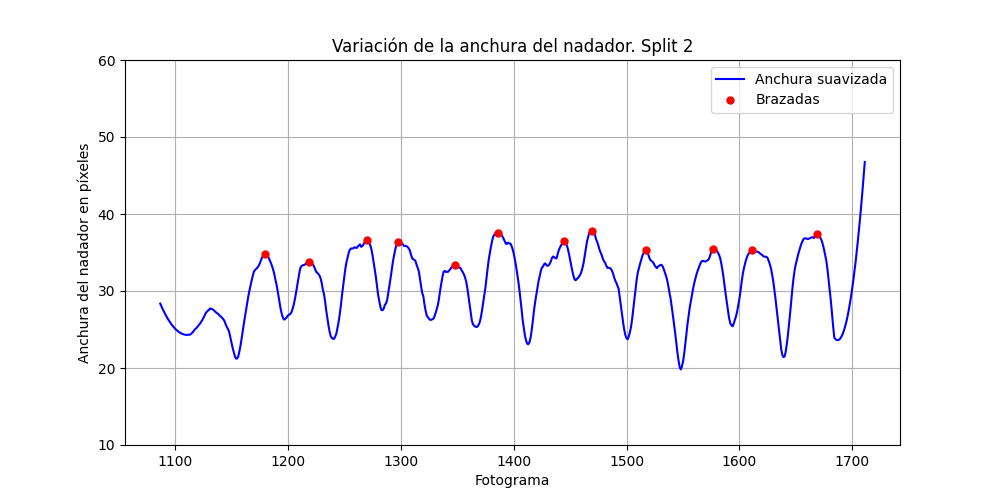
\includegraphics[scale=0.2]{imagenes/anchuras_calle_5_freestyle_YOLO.png}
                        \\ a) Nado en mariposa & b) Nado en crol
                    \end{tabular}
                \caption{Variaciones de anchura para distintos estilos de nado.}
                \label{fig:ejemplovariacionanchura}
            \end{figure}
        \end{frame}
        
        %%%%%%%%%%%%%%%%%%%%%%%
        \subsection{Cálculo de la frecuencia media de nado}
        \begin{frame}{Cálculo de la frecuencia media de nado}
            Podemos calcular la frecuencia media de nado por split (FNMS) haciendo uso de:
            \begin{equation}
                \text{FNMS} (brazadas/min) = \frac{ \text{número de brazadas} * \frac{\text{60 segundos}}{minuto} }{ \text{segundos en recorrer la región de interés}}
            \end{equation}
            La frecuencia de nado media para toda la secuencia de vídeo será la media aritmética de las FNMS.
        \end{frame} 
        
        %%%%%%%%%%%%%%%%%%%%%%%
        \subsection*{Evaluación experimental}
        \begin{frame}{Valores de referencia} 
            Dado que no se disponía de etiquetas, se ha medido manualmente el tiempo empleado en recorrer cada región de interés y el número de brazadas realizado.
            
            Se han usado 14 splits: 4 para nado en estilo mariposa, 4 en crol, 4 en braza y 2 en espalda.
        \end{frame}
        
        \begin{frame}{¿Cómo determinar el error en las predicciones?}
            Se hace uso del error absoluto relativo, cuya expresión es: \\
            \begin{equation}
                Error_{\text{absoluto relativo}} = \frac{|Valor_{real} - Valor_{predicho}|}{Valor_{real}}
            \end{equation}
            \\Nos permite tener en cuenta los valores reales al calcular el nivel de error de la predicción. Podemos comparar entre vídeos.
        \end{frame} 

    \begin{frame}{Errores en la predicción del tiempo empleado por split}
        \begin{table}
            \centering
            \small
            \begin{tabular}{|c|c|c|} \hline
             Estilo & Err. relatv. medio GSoC & Err. relatv. medio YOLO  \\ \hline
             Mariposa & \textbf{0.024803} & 0.026495 \\
             Crol & 0.061423 & \textbf{0.02374}  \\   
             Braza & 0.043430 & \textbf{0.029135} \\
             Espalda & 0.017900 & \textbf{0.016695} \\
             Media & 0.039603 & \textbf{0.025062} \\ \hline
            \end{tabular}
            \caption{Comparativa entre los errores absolutos relativos medios de los tiempos estimados.}
            \label{tab:tablatiemposmedioscap5}
        \end{table}
        YOLO proporciona errores de predicción menores, aunque son pequeños en todo caso.
    \end{frame}
    
    \begin{frame}{Errores en la predicción del número de brazadas}
        \begin{table}
            \centering
            \begin{tabular}{|c|c|c|} \hline
             Estilo & Err. relatv. medio GSoC & Err. relatv. medio YOLO  \\ \hline
             Mariposa & 0.0486 & \textbf{0.0208} \\
             Crol & 0.0941 & \textbf{0}  \\   
             Braza & 0.1847 & \textbf{0.0208} \\
             Espalda & 0.2765 & \textbf{0.0417} \\
             Media & 0.1330 & \textbf{0.0178} \\ \hline
            \end{tabular}
            \caption{Comparativa entre los errores relativos medios del número de brazadas estimadas.}
            \label{tab:tablaerroresmediosbrazadas}
        \end{table}
        YOLO ofrece menores errores de predicción, los cuales GSoC suele cometer y pueden llegar a ser realmente flagrantes.
    \end{frame}

    
    \begin{frame}{Errores de predicción de la frecuencia media de nado}
        \begin{table}
            \centering
            \begin{tabular}{|c|c|c|} \hline
                Estilo & Err. relatv. medio GSoC & Err. relatv. medio YOLO  \\ \hline
                Mariposa & 0.0540 & \textbf{0.0467} \\
                Crol & 0.1093 & \textbf{0.0247}  \\   
                Braza & 0.1574 & \textbf{0.0417} \\
                Espalda & 0.2764 & \textbf{0.0436} \\
                Media & 0.1311 & \textbf{0.0385} \\ \hline
            \end{tabular}
            \caption{Comparativa entre los errores relativos medios de las frecuencias medias de nado estimadas.}
            \label{tab:tablaerroresmediosprediccionesfrecuencia}
        \end{table}
        GSoC puede llegar a cometer grandes errores en función del estilo de nado. YOLO ofrece un rendimiento superior y predicciones más consistentes.
    \end{frame}

    %%%%%%%%%%%%%%%%%%%%%%%
    \section{Conclusiones y trabajo futuro}
    
        \begin{frame}{Conclusiones}
            \begin{itemize}
                \item La banda de crominancia roja de YCbCr y el algoritmo de sustracción de fondos GSoC permiten detectar al nadador de manera aceptable.
                \item YOLOv4 realiza detecciones más precisas que las técnicas clásicas de imágenes, aunque para ello necesita de mayor tiempo de ejecución.
                \item El método propuesto permite realizar una estimación bastante cercana a la realidad de la frecuencia media de nado si se utiliza YOLO como detector.
            \end{itemize}
        \end{frame}
        
        \begin{frame}{Trabajo futuro}
            \begin{itemize}
                \item Uso de nuevos algoritmos de sustracción de fondos.
                \item Uso de nuevas versiones de YOLO y conjuntos de imágenes de entrenamiento más variados.
                \item Entrenar y utilizar YOLO sobre imágenes representadas haciendo uso de las bandas de crominancia del espacio de color YCbCr puede resultar prometedor.
            \end{itemize}
        \end{frame}
        
        \begin{frame}[standout]
            \textbf{{\Huge FIN}}
            \noindent\rule[-1ex]{\textwidth}{1.5pt}\\[3.5ex]
            ¿Alguna duda o pregunta?
        \end{frame}

    
\end{document}